\documentclass[12pt,a4paper]{article}
\usepackage[spanish]{babel}
\usepackage[utf8]{inputenc}
\usepackage{graphicx}% Include figure files
%\usepackage{dcolumn}% Align table columns on decimal point
\usepackage{bm}% bold math
\usepackage[]{hyperref}
\hypersetup{colorlinks=true,}
\usepackage{standalone}
\usepackage{color}
\usepackage{mathrsfs}
%\usepackage{amsthm}
\usepackage{pst-plot}
\usepackage{pstricks-add} 
\usepackage{wrapfig}
\usepackage{cancel}
\usepackage{amssymb}
\usepackage{latexsym}
\usepackage{epsfig}
\usepackage{enumitem}
\usepackage{float}
\usepackage{physics}
\usepackage{algorithm,algpseudocode}
\usepackage{tikz, tkz-euclide}
\usetikzlibrary{shapes,arrows,spy,positioning,snakes}
\newcommand\numberthis{\addtocounter{equation}{1}\tag{\theequation}}
\usepackage{makeidx}
\usepackage[margin=1.3cm]{geometry}
\renewcommand{\baselinestretch}{1}
\usepackage[colorinlistoftodos]{todonotes}
\usepackage{cleveref}
\usepackage{neuralnetwork}
\usepackage[utf8]{inputenc}
\usepackage[spanish]{babel}
\usepackage{amsmath}
\usepackage{tikz}
\usetikzlibrary{babel}
\usepackage{bigints}
\usepackage{float}  
\usepackage{subcaption}
\captionsetup[subfigure]{labelformat=empty}
\usepackage{cancel}
\usepackage{amsthm,amssymb,amsfonts}
\usepackage{tikz,lipsum,lmodern}
\usepackage[most]{tcolorbox}

\newcommand{\R}{\mathbb{R}} 

\usepackage[utf8]{inputenc}


\begin{document}

\newcommand{\pr}[1]{\left( #1 \right)}
\newcommand{\nr}[1]{\left| #1 \right|}
\newcommand{\cc}[1]{\cancel{#1}}
\newcommand{\dx}[1]{\dfrac{d#1}{dx}}

\begin{center}
{\Large\textbf{Ecuaciones Diferenciales I}}\\
\vspace{3mm}
{\Large \bf Tarea 1}\\
\vspace{3mm}
\begin{large} Israel Tomás Cuevas Carmona,\end{large}\\
\begin{large} Ximena Cruz Nava,\end{large}\\
\begin{large} Luis Enrique Velázquez Pérez,\end{large}\\
\begin{large} Sebastián Calderón Alba,\end{large}\\
\begin{large}\textit{Miguel Eduardo Jaime Velázquez}\end{large}
\end{center}
{\bf Instrucciones}: Resuelve los problemas en hojas en blanco, con letra legible y buena presentación. Se calificará el procedimiento. Se entrega en equipos de máximo 6 personas. 

%%%%%% Resolver los problemas en el apartado del problema que aparece a la izquierda  <-----  %%%%%%%

\begin{enumerate}
    \item Demuestre que las siguientes ecuaciones no son exactas, encuentra el factor integrante que las vuelve exactas y resuelve los PVI.
\end{enumerate}
\begin{enumerate}
    \item[a)] $(10-6y+e^{-3x})\dd x- 2 \dd y=0, \qquad y(0)=1$
\begin{align*}
(10-6y+e^{-3x})\dd x- 2 \dd y=0, \qquad y(0)=1
\end{align*}
\end{enumerate}
Una ecuación diferencial es exacta si $F(x,y)$ tal que en el dominio se cumple que:
\begin{align*}
    \frac{\partial F}{\partial x} &= P(x,y)\\
    \frac{\partial F}{\partial y} &= Q(x,y)
\end{align*}
Es fácil ver que $\displaystyle \frac{\partial P}{\partial y} \neq \frac{\partial Q}{\partial x}$, por lo tanto debemos buscar un factor integrante
\begin{align*}
    P(x,y)&= 10-6y+e^{-3x}\\
    Q(x,y)&= -2
\end{align*}
Resolviendo la derivada parcial
\begin{align*}
    \frac{\frac{\partial P}{\partial y} - \frac{\partial Q}{\partial x}}{Q} & = 3
\end{align*}
Por lo tanto
\begin{equation*}
    \mu (x) = e^{\int 3 dx} \implies e^{3x}
\end{equation*}
Resolviendo con el factor integrante, tenemos que
\begin{align*}\label{sol:1}
    e^{3x}[(10-6y+e^{-3x})dx - 2dy]&= 0\\
    e^{3x}(10-6y+e^{-3x})dx-2e^{3x}dy &= 0 \numberthis
\end{align*}
Resolviendo de nuevo las derivadas parciales en \ref{sol:1} tenemos que:
\begin{align*}
    \frac{\partial P}{\partial x} &= -6e^{3x} \\
    \frac{\partial Q}{\partial y} &= -6e^{3x}
\end{align*}
Por lo tanto $P = Q$, entonces es exacta.\\
Dividiendo por $dx$ y reescribiendo la ecuación tenemos que:
\begin{align*}
    \dv{x}{y} +3y =\frac{e^{-3x}}{2} +5.
\end{align*}
Multiplicando por el factor integrante
\begin{align*}
    (e^{3x})\dv{y(x)}{x} + \dv{(e^{3x})}{x}y(x) &= (e^{3x}) \frac{e^{-3x}}{2} +5\\
     \int \dv{(e^{3x})y(x)}{x} \dd x &= \frac{1}{2} \int \dd x + 5 \int e^{3x}\dd x \\
     e^{3x} y & = \frac{x}{2}+\frac{5}{3}e^{3x}+C\\
     y & = \frac{x}{2e^{3x}}+\frac{5}{3}+\frac{C}{e^{3x}}\\
\end{align*}
Obteniendo el PVI para $y(0)=1$
\begin{align*}
    c = - \frac{2}{3}
\end{align*}
Entonces la solución particular es 
\begin{center}
    \fbox{$y = \dfrac{x}{2e^{3x}}- \dfrac{2}{3e^{3x}}+\dfrac{5}{3}$}
\end{center}




\begin{itemize}
    \item[b)] $\cos x \dd x+ \left( 1 + \frac{2}{y} \right) \sen x \dd y=0, \qquad y(0)=2$
\end{itemize}
\begin{align*}
    \underbrace{\cos x}_{M\pr{x,y}} \dd x+\underbrace{ \left( 1 + \frac{2}{y} \right) \sen x }_{N\pr{x,y}}\dd y=0, \qquad y(0)=2
\end{align*}

Verifiquemos si se trata de una ecuación exacta, recordando que para que lo sea se debe cumplir que $\dfrac{\partial M}{\partial y}=\dfrac{\partial N}{\partial x}$, en este caso

\begin{align*}
    \dfrac{\partial M}{\partial y} &= \dfrac{\partial}{\partial x} \cos x = 0 \\
    \dfrac{\partial N}{\partial x}&=\dfrac{\partial}{\partial x}\left(1+\dfrac{2}{y}\right)\sen x = \left(1+\dfrac{2}{y}\right)\cos x  \neq 0 \\
    \therefore \dfrac{\partial M}{\partial y} &\neq \dfrac{\partial N}{\partial y}
\end{align*}
 
 Por lo tanto la ecuación no es exacta. Ahora vamos a encontrar un factor integrante, para lo cual multiplicaremos toda la ecuación por este factor, al cual llamaremos $\mu$, lo importante de este factor es que al agregarlo convertiremos nuestra ecuación no exacta a una exacta 
 
 \begin{align*}
     \mu \cos x \dd x + \mu \pr{1+\dfrac{2}{y}}\sen x \dd y = 0
 \end{align*}
 
 Para que sea exacta se debe cumplir que
 
 \begin{align*}
     \dfrac{\partial}{\partial y} \mu \cos x &= \dfrac{\partial}{\partial x} \mu \pr{1+\dfrac{2}{y}}\sen x \\ 
     \Rightarrow \cos x \dfrac{\partial}{\partial y} \mu + \mu \cc{\dfrac{\partial }{\partial y} \cos x} &= \pr{1+\dfrac{2}{y}}\pr{\sen x \dfrac{\partial}{\partial x}\mu + \mu \dfrac{\partial}{\partial x}\sen x} \\
     \Rightarrow \cos x \dfrac{\partial \mu}{\partial y} &= \pr{1+\dfrac{2}{y}}\pr{\sen x\dfrac{\partial \mu}{\partial x}+\mu \cos x}
 \end{align*}
 
 Para simplificar un un poco la última ecuación, supondremos que $\mu=\mu\pr{x}$, por lo que tenemos
 
 \begin{align*}
     0&=\pr{1+\dfrac{2}{y}}\pr{\sen x \dfrac{\partial \mu}{\partial x}+\mu\cos x} \\ 
     \Rightarrow \sen x \dfrac{\partial \mu}{\partial x} &= -\mu \cos x \\
     \Rightarrow \int \dfrac{d\mu}{\mu} &= -\int\dfrac{\cos x}{\sen x} \dd x \\ 
     \Rightarrow \ln \nr{\mu} &= -\ln\nr{\sen x} \\ 
     \therefore \mu &= \dfrac{1}{\sen x}
 \end{align*}
 
 Ahora verifiquemos que con el factor integrante la ecuación es exacta
 
 \begin{align}
     \underbrace{\dfrac{\cos x}{\sen x}}_{M\pr{x,y}}\dd x + \underbrace{\pr{1+\dfrac{2}{y}}\cc{\dfrac{\sen x}{\sen x}}}_{N\pr{x,y}}\dd y &= 0
 \end{align}
 
 Calculemos $M_y$ y $N_x$
 
 \begin{align}
     \dfrac{\partial }{\partial y} \dfrac{\cos x}{\sen y} &= 0\\
     \dfrac{\partial}{\partial x} \pr{1+\dfrac{2}{y}}&= 0 \\
     \therefore \dfrac{\partial M}{\partial y} = \dfrac{\partial N}{\partial x}
 \end{align}
 
 Ya tenemos una ecuación exacta, que además podemos ver que es separable
 
 \begin{align*}
     \Rightarrow \dfrac{\cos x}{\sen x}\dd x&=-\pr{1+\dfrac{2}{y}} \dd y\\
     \int \dfrac{\cos x}{\sen x} \dd x &= -\int \dd y -2\int\dfrac{\dd y}{y} \\ \Rightarrow \ln \nr{\sen x} + C_1 &= -y -2\ln\nr{y} +C_2 \\ 
     \Rightarrow \sen x &= e^{-y-2\ln\nr{y}}C_3 ~~~~~~~~~~~~~ \text{con $C_3=e^{C_2-C_1}$} \\
     \Rightarrow \sen x&= \dfrac{C_3}{e^y y^2}
 \end{align*}
 
 \begin{center}
     \fbox{$\therefore e^y y^2 = \dfrac{C}{\sen x}$}
 \end{center}
 
 Aplicando el PVI $x=0$, $y=2$ 
 
 \begin{align*}
     0&=\dfrac{C_3}{4e^2} \\
     \therefore C_3 &= 0
 \end{align*}
 
Veamos que para la condición inicial de $x=0$  tenemos un caso degenerado ya que $\sen x=0 \Rightarrow x=m\pi,~~~~~m\in \mathbb{Z}$  Es decir, la soluciones quedan como lineas verticales paralelas con periodo $\pi$ 


\begin{enumerate}
    \item[2.] Resuelve el PVI asociado a la ecuación separable
\end{enumerate}

\begin{enumerate}
   
      \item[a)] 
\begin{align*}
    \dv{y}{x}= \frac{(y^{2}-y)x}{x^{2}+1}, \quad y(0)=2
\end{align*}

Vamos a comenzar separando las ecuaciones 

\begin{align*}
    \dfrac{1}{y^2-y}dy=\dfrac{x}{x^2+1}dx
\end{align*}

Ahora vamos a integrar

\begin{align*}
    \int \dfrac{1}{y^2-y}dy&=\int\dfrac{x}{x^2+1}dx\\
    \Rightarrow \int\dfrac{1}{y^2\pr{1-\frac{1}{y}}}dy&=\int\dfrac{x}{x^2+1}dx
\end{align*}

Para integrar el miembro izquierdo haremos el cambio de variable $u=1-\dfrac{1}{y}$, $du=\dfrac{1}{y^2}dy$. Por otro lado, para integrar el miembro derecho haremos el cambio de variable $w=x^2+1$, $dw=2xdx$

 \begin{align*}
 \Rightarrow \int\dfrac{du}{u} &= \dfrac{1}{2}\int \dfrac{dw}{w}\\
 \Rightarrow \ln \nr{u} + C_1 &= \dfrac{1}{2}\ln \nr{w} + C_2 \\
 \Rightarrow \ln \nr{1-\dfrac{1}{y}} &= \dfrac{1}{2} \ln \nr{x^2+1} + C_2-C_1 
 \end{align*}
 
 Aplicando la función exponencial y haciendo $C_3=C_2-C_1$
 
 \begin{align*}
     \exp\pr{\ln\nr{1-\dfrac{1}{y}}}&=\exp\pr{\ln\nr{x^2+1}^{1/2}+C_3} \\
     \Rightarrow 1-\dfrac{1}{y}&= \pr{x^2+1}^{1/2}e^{C_3} \\
     \Rightarrow  \dfrac{1}{y} &= 1-C\pr{x^2+1}^{1/2} \\
     \therefore y &= \dfrac{1}{1-C\sqrt{x^2+1}}
 \end{align*}
 
 Aplicando el PVI 
 
 \begin{align*}
     y\pr{0}=\dfrac{1}{1-C\sqrt{0+1}}&=2 \\ 
     \Rightarrow  \dfrac{1}{1-C}&=2 \\ 
     \Rightarrow \dfrac -{1}{2}&=C-1 \\ 
     \therefore C &= \dfrac{1}{2}
     \end{align*}
     
Por lo que ahora tenemos que la función $y$

\begin{align*}
    y=\dfrac{1}{1-\frac{1}{2}\sqrt{x^2+1}}=\dfrac{2}{2-\sqrt{x^2+1}}
\end{align*}
     
     \begin{center}
         \fbox{$\therefore y=\dfrac{2}{2-\sqrt{x^2+1}}$}
     \end{center}

 

    \item[b)]
\begin{align*}
    (1+x^{4})\dv{y}{x}=-x(1+4y^{2}), \quad y(1)=0
\end{align*}

Vamos a comenzar separanddo las ecuaciones 

\begin{align*}
    \dfrac{dy}{1+4y^2}=-\dfrac{xdx}{1+x^4}
\end{align*}

Ahora vamos a integrar

\begin{align*}
    \int \dfrac{1}{1+4y^2}=-\int \dfrac{x}{1+x^4}dx
\end{align*}

Para integrar el miembro izquierdo haremos el cambio de variable $u=2y$, $du=2dy$ y para integrar el miembro derecho haremos $w=x^2$, $dw=2xdx$

\begin{align*}
    \Rightarrow \dfrac{1}{2}\int \dfrac{1}{1+u^2} du &= -\dfrac{1}{2}\int \dfrac{1}{1+w^2}dw \\
    \Rightarrow \dfrac{1}{2} \arctan \pr{u} + C_1 &= -\dfrac{1}{2}\arctan\pr{w}+C_2 \\ 
    \Rightarrow \cc{\dfrac{1}{2}} \arctan\pr{2y} &= -\cc{\dfrac{1}{2}}\arctan\pr{x^2}+C_2-C_1 \\ 
    \Rightarrow \arctan\pr{2y}&=-\arctan\pr{x^2}+2\pr{C_2-C_1}
\end{align*}

Haremos $C=2\pr{C_2-C_1}$ y aplicaremos la función tangente, sin olvidar que la función arcotangente es impar

\begin{align*}
    \Rightarrow \tan\pr{\arctan\pr{2y}}&=\tan\pr{\arctan\pr{-x^2}+C} 
\end{align*}

Ahora, recordemos la identidad $\tan\pr{\alpha+\beta}=\frac{\tan\alpha+\tan\beta}{1-\tan\alpha\tan\beta}$

\begin{align*}
    \Rightarrow 2y &= \dfrac{\tan\pr{\arctan\pr{-x^2}}+\tan C}{1-\tan\pr{\arctan\pr{-x^2}}\tan{C}} \\
    &=\dfrac{C_f - x^2}{1+C_f x^2}
\end{align*}

Con $C_f=\tan C$. Ya tenemos la solución de la ecuación diferencial

\begin{align*}
    \therefore y = \dfrac{C_f-x^2}{2+2C_fx^2}
\end{align*}

Ahora resolvamos el PVI

\begin{align*}
    y\pr{1}&=\dfrac{C_f-1}{2+2C_f\pr{1}}=0 \\
    \Rightarrow C_f=1
\end{align*}

Por lo que ahora tenemos que la función $y$

\begin{align*}
    y=\dfrac{1-x^2}{2+2x^2}
\end{align*}

\begin{center}
    \fbox{$\therefore y=\dfrac{1}{2}\pr{\dfrac{1-x^2}{1+x^2}}$}
\end{center}





\end{enumerate}
\begin{enumerate}
    \item[3.] Resuelve la ecuación homogénea 
\end{enumerate}
%\begin{align*}
%    (-y^{3}+x^{3}) \dd x - xy^{2} \dd y = 0
%\end{align*}
%\begin{align*}
%    (x^{2}y^{3}+x^{5}) \dd x +(x^{3}y^{2}+y^{5}) \dd y = 0, \qquad %y(1)= 2
%\end{align*}

\begin{itemize}
    \item[a)] $(-y^3+x^3)dx-xy^2dy=0$
    \begin{enumerate}
     \item Verificamos si es homogénea y de que grado es:\\
    $M=-y^3+x^3$ \hspace{.3cm} y  \hspace{.3cm}$N=xy^2$  \hspace{1cm} Cumplen con ser homogénea y ambas son de grado 3
    \item Realizamos un cambio de variable: $y=ux$\hspace{1cm} $dy=udx+xdu$\hspace{1cm} $\frac{y}{x}=u$
    \item Sustituimos en la ecuación inicial:
    \begin{align*}
        (x^3-u^3x^3)dx+xu^2x^2(udx+xdu) &= 0\\
        x^3dx-\cc{u^3x^3dx}+\cc{u^3x^3dx}+x^4u^2du &= 0\\
        x^3dx+x^4u^2du &= 0
    \end{align*}
    Y ahora resolvemos por variables separables:
    \begin{align*}
        x^3dx &= -x^4u^2du \\
        \frac{x^3}{x^4}dx &= -u^2du\\
        \frac{1}{x}dx  &= -u^2du\\
        \int\frac{1}{x}dx &= -\int u^2du \\
        \ln (x) &= -\frac{u^3}{3}+c
    \end{align*}
    Sustituimos $u$ y así volver a nuestro contexto original y despejamos $y$:
    \begin{align*}
        \ln (x) &= -\frac{\left(\frac{y}{x}\right) ^ 3}{3}+c \\
        \ln (x) &= -\frac{y^3}{3x^3}+c \\
        \therefore y &= \sqrt[3]{3x^3(c-\ln (x))}
    \end{align*}
    
    \begin{center}
        \fbox{$\therefore y = \sqrt[3]{3x^3(c-\ln (x))}$}
    \end{center}
    
    
     \end{enumerate}
    
    
    
    
    
     \item[b)] $(x^2y^3+x^5)dx + (x^3y^2+y^5)dy=0$, \hspace{1cm} $y(1)=2$
     \begin{enumerate}
         \item Verificamos que sea homógenea y de que grado es:\\
         $M=x^2y^3+x^5$\hspace{.3cm} y \hspace{.3cm} $N=x^3y^2+y^5$ \hspace{.3cm}  Cumplen con ser homogénea y ambas son de grado 5
         \item Resolvemos:\\
         Si dividimos la ecuación entre $\left((y+x)(y^2-xy+x^2)\right)$ obtenemos:
         \begin{equation*}
             y^2dy+x^2dx=0
         \end{equation*}
         La cual podemos resolver por variables separables:
         \begin{align*} 
             y^2dy  &= -x^2dx\\
             \int y^2dy &= - \int x^2dx\\
             \frac{y^3}{3}  &= - \frac{x^3}{3} + c
         \end{align*}
Despejando para $y$ y  $c$ : \hspace{1cm} $y = \sqrt[3]{c-x^3}$ \hspace{2cm}  $c = y^3- x^3$
       \item Resolviendo el PVI  \hspace{1cm}$y(1)=2$ \\
       $\Rightarrow$ \hspace{1cm} $c=7$ \hspace{4cm}$\therefore$\hspace{.2cm} $y=\sqrt[3]{7-x^3}$
       
       \begin{center}
           \fbox{$\therefore y=\sqrt[3]{7-x^3}$}
       \end{center}
       
       
     \end{enumerate}
\end{itemize}
\begin{enumerate}
    \item[4.] Resuelve el PVI
\end{enumerate}

\begin{enumerate}
\item[a)]
\begin{align*}
    \dv{y}{x} = (x+y+1)^{2}, \qquad y(0)=0
\end{align*}

Vamos a hacer el cambio de variable $u=x+y+1$ de modo que tenemos 

\begin{align*}
    \dx{u}&=1+\dx{y}\\
    \Rightarrow \dx{y}&=\dx{u}-1
\end{align*}

De modo que sustituyendo en la ecuación original

\begin{align*}
    \dx{u}-1&=u^2\\
    \Rightarrow \dfrac{1}{u^2+1}&=dx
\end{align*}

Integrando

\begin{align*}
    \int\dfrac{1}{u^2+1}&=\int dx\\
    \Rightarrow \arctan\pr{u}+C_1&=x+C_2\\
    \Rightarrow \tan\pr{\arctan\pr{u}}&=\tan\pr{x+C_2-C_1}  ~~~~~~~~~~~~~~ \text{haciendo  } C_3=C_2-C_1 \\
    \Rightarrow u&=\tan\pr{x+C_3} ~~~~~~~~~~~~~~~~~~~~~ \text{sustituyamos $u=x+y+1$}\\
    \Rightarrow x+y+1&=\tan\pr{x+C_3}\\
    \therefore y&=\tan\pr{x+C_3}-x-1
\end{align*}

Resolviendo el PVI tenemos

\begin{align*}
    y\pr{0}&=\tan\pr{C_3}-1=0\\
    \Rightarrow C_3&=\arctan\pr{1}\\
    \therefore C_3&=\dfrac{\pi}{4}
\end{align*}

Por lo que la solución queda como

\begin{center}
    \fbox{$\therefore y=\tan\pr{x+\dfrac{\pi}{4}}-\pr{x+1}$}
\end{center}

Podemos ver también la  solución, utilizando la identidad $\tan\pr{\alpha+\beta}=\frac{\tan\alpha+\tan\beta}{1-\tan\alpha\tan\beta}$,  como

\begin{align*}
    y=-\pr{\dfrac{\tan\pr{x}+1}{\tan\pr{x}-1}+x+1}
\end{align*}


\item[b)]

\begin{align*}
    \dv{y}{x} = \frac{4x-7y}{-4x+7y-5}, \qquad y(0)=1
\end{align*}

Para resolver este problema vamos a proponer el cambio de variable $u=-4x+7y-5$, de donde nos resultan las siguientes igualdades 

\begin{align*}
    \dx{u}&=7\dx{y}-4\\
    4x-7y&=-u-5
\end{align*}

Por lo que sustituyendo en la ecuación original tenemos

\begin{align*}
    \dfrac{1}{7}\pr{\dx{u}+4}&=\dfrac{-\pr{u+5}}{u}\\
    \Rightarrow  \dx{u}&=\dfrac{-7\pr{u+5}}{u}-4=\dfrac{-7u-35-4u}{u}\\
    \Rightarrow  \dx{u}&=\dfrac{-\pr{11u+35}}{u} \\ 
    \Rightarrow \dfrac{u}{11u+35}du&=-dx
\end{align*}

Para integrar el miembro izquierdo haremos el cambio de variable $w=11u+35$, lo que nos resulta que $u=\dfrac{1}{11}\pr{w-35}$ y $\dfrac{dw}{11}=du$, por lo que tenemos

\begin{align*}
    \dfrac{1}{121}\int\dfrac{w-35}{w}dw&=-\int dx \\ 
    \Rightarrow \dfrac{1}{121}\pr{\int dw - 35 \int \dfrac{dw}{w}  }&=-x+C_2 \\ 
    \dfrac{1}{121}\pr{w-35\ln\nr{w}}+C_1&=-x+C_2
\end{align*}

Sustituyendo $w=-44x+77y-20$ y haciendo $C=121(C_2-C_1)$ tenemos

\begin{align*}
    -44x+77y-20-35\ln\nr{-44x+77y-20}&=-121x+C \\
    \Rightarrow 35\ln \nr{-44x+77y-20}&=77x+77y+C_f  ~~~~~~~~~~~~ \text{con $C_f=-C-20$} 
\end{align*}

Vamos a aplicar el PVI, haciendo $x=0$, $y=1$

\begin{align*}
    35\ln\nr{77-20}&=77+C_f\\
   \therefore C_f &= 35\ln\nr{57}-77
\end{align*}

Por lo que la solución al problema queda expresada como 

\begin{align*}
    \ln\nr{-44x+77y-20}&=\dfrac{77}{35}\pr{x+y-1}+\ln\nr{57} \\
    \Rightarrow \ln\nr{-44x+77y-20}-\ln\nr{57}&=\dfrac{77}{35}\pr{x+y-1}
\end{align*}

\begin{center}
    \fbox{$\therefore \ln\nr{\dfrac{-44x+77y-20}{57}}=\dfrac{77}{35}\pr{x+y-1}$}
\end{center}



\end{enumerate}

\begin{enumerate}
    \item[5.] Resuelve la ecuación de Ricatti con valores iniciales
\end{enumerate}
\begin{enumerate}
    \item[a)] $y'=3t^{-2}-t^{-4}+2(t^{-1}-t^{-3})y-t^{-2}y^{2}, \qquad y(1)= - \frac{1}{2}, \qquad y_{1}(t)=-\frac{1}{t}$
\end{enumerate}
\begin{align*}
    y' = \underbrace{3t^{-2}-t^{-4}}_{q_{1}(x)}+\underbrace{2(t^{-1}-t^{-3})}_{q_{2}(x)}y_{1}-\underbrace{t^{-2}}_{q_{3}(x)}y_{1}^{2}, \quad y(1)= - \frac{1}{2}, \quad y_{1}(t)=-\frac{1}{t}
\end{align*}
Tiene la forma de la ecuación de Ricatti
\begin{align*}
    y=y_{1}+\frac{1}{2} & \implies y'=y_{1}'-\frac{z'}{z^{2}}\\
    y = -\frac{1}{t}+\frac{1}{2} & \implies y'= -\frac{t'}{t^{2}}- \frac{z'}{z^{2}}
\end{align*}
\begin{align*}
    \left( -\frac{t}{t^{2}}- \frac{z'}{z^{2}} \right)= 3t^{-2}-t^{-4}+2(t^{-1}-t^{-3})\left( -\frac{1}{t}+\frac{1}{2} \right) -t^{-2} \left( -\frac{1}{t}+\frac{1}{2} \right)^{2}
\end{align*}
Sabemos que $y_{1}'$ es solución. Por la forma llegada en clase
\begin{align*}
    z' +\left(2q_{3}(x)y_{1}+q_{2}(x)\right)z&=-q_{3}(x)
    & & \text{Sustituyendo}\\
    z' + \left(2(-t^{-2})\left( -\frac{1}{t}\right)+2(t^{-1}-t^{-3}\right)z & =-t^{-2}
    & &  \text{Una ecuación lineal }p(t)
\end{align*}
Por lo visto en clase la solución de esta ecuación
\begin{align*}
    \mu(t) = e^{\int p(t)dt} & \implies \frac{2t^{-2}}{t}+2t^{-1}-2t^{-3}=p(t)\\
    & \implies \int p(t)\dd t = 2\int \frac{1}{t^{3}}\dd t + 2t^{-1}-2t^{-3} \dd t\\
    & \implies 2\int t^{-3}\dd t + 2 \int t^{-1} \dd t - 2\int t^{-3} \dd t\\
    & \implies 2 \int t^{-1} \dd t \\
    & \implies 2 \ln \mid t \mid + C 
\end{align*}
Regresando, $\displaystyle e^{\left({\int p(t) \dd t}\right)} = e^{\left( 2 \ln \mid t \mid + C \right)} \implies e^{(2 \ln \mid t \mid)} \cdot e^{C} = t^{2} e^{C}$\\

Volviendo a la ecuación lineal, donde $c=0$, resolviendo por factor integrante
\begin{align*}
    t^{2}\cdot z' + t^{2}\left( \frac{2t^{2}}{2} +2t^{-1} -2t^{-3} \right) = t^{2}(-t^{-2}) \implies t^{2}\left( \frac{-1}{t^{2}}\right) = -1
\end{align*}
\begin{align*}
    t^{2}z = \int -1dt \implies t^{2}z= -t + C
\end{align*}
Regresando a la original
\begin{align*}
    y  & = - \frac{1}{t}+ \frac{1}{2}\\
    y + \frac{1}{t} & \implies z = \frac{1}{y+\frac{1}{t}}\\
    & \implies \frac{1}{y+\frac{1}{t}} = -t+ C 
    & & \text{Es la solución general.}
\end{align*}
Para nuestra C, tenemos que $y(1)= -\frac{1}{2}$
\begin{align*}
    \frac{1}{-\frac{1}{2}+\frac{1}{1}}=-1+C \implies \frac{1}{\frac{1}{2}}= -1+C \implies 2+1 = C = 3
\end{align*}
Para la solución general $\displaystyle \frac{1}{y+\frac{1}{t}}=-t+3$
\begin{align*}
    y = \frac{1}{-t+3}- \frac{1}{t}
\end{align*}
\begin{enumerate}
    \item[b)] $y'= - (t^{2}+6t+4)+2(t+3)y-y^{2}, \qquad y(1)= \frac{5}{2}; \qquad y_{1}(t)=t+1$
\end{enumerate}
\begin{align*}
    y'= - \underbrace{(t^{2}+6t+4)}_{q_{1}(x)}+\underbrace{2(t+3)}_{q_{2}(x)}y-\underbrace{1}_{q_{3}(x)}y^{2}, \quad y(1)= \frac{5}{2}; \quad y_{1}(t)=t+1
\end{align*}
Podemos ver que si cumple la forma de Ricatti\\

Sea $\displaystyle y=y_{1}+\frac{1}{2} \implies y=(t+1)+\frac{1}{2} \implies y' = (t+1)+\frac{1}{2} \implies y'=(t+1)'+\frac{z'}{z^{2}}= 1 + \frac{z'}{z^{2}}$
Sustituyendo
\begin{align*}
    \left( 1 + \frac{z'}{z^{2}}\right) = - \underbrace{(t^{2}+6t+4)}_{q_{1}(x)}+\underbrace{2(t+3)}_{q_{2}(x)}\left( t+1+\frac{1}{2} \right)-\underbrace{1}_{q_{3}(x)}\left( t+1+\frac{1}{2} \right)^{2}
\end{align*}
$y_{1}'$ es solución. Por lo que usando la forma a la que se llegó
\begin{align*}
    z'+(2q_{3}(x)\cdot y_{1}+q_{2}(x))\cdot 2 & = -q_{3}(x)\\
    z'+(2\cdot-1\cdot(t+1)+2(t+3))\cdot2&=-1\\
    z' +(-2t-2+2t+6)\cdot 2 &= -1\\
    z'+4z & = -1
    & & \text{Ya es lineal}
\end{align*}
Usando $\displaystyle \mu(t)=e^{\int p(t)dt} \implies \int 4 dt = 4t$
\begin{align*}
    4t\cdot z' + 4t(4z)=-4t & \implies 4tz'+16tz=-4t\\
    & \implies 4 tz = \implies - \int 4t dt\\
    & \implies -4 \frac{t^{2}}{2} + C = 4tz\\
    & \implies -2t^{2}=4tz\\
    & \implies z = -\frac{2t^{2}}{4t} + C\\
    & \implies - \frac{t}{2}+C = 2
\end{align*}
De $\displaystyle y=\frac{1}{2}+t+1$ tenemos
\begin{align*}
    y-t-1 = \frac{1}{2} &\implies \frac{1}{y-t-1}=2\\
    & \implies \frac{1}{y-t-1}= - \frac{t}{2}+ C\\
    & \implies \frac{1}{-\frac{t}{2}+ C}=y-t-1\\
    & \implies y = \frac{1}{-\frac{t}{2}+ C}-t-1
    & & \text{Forma implícita}
\end{align*}
Si $y(1)= \frac{5}{2}$
\begin{align*}
    \frac{5}{2}= \frac{1}{-\frac{1}{2}+ C}-1-1 & \implies \frac{5}{2}= \frac{1}{-\frac{1}{2}+ C}-2\\
    & \implies \frac{5}{2}-2 = \frac{1}{2} + C\\
    & \implies \frac{1}{2} = \frac{1}{\frac{1}{2}+C}\\
    & \implies \frac{1}{2}+ C = 2\\
    & \implies C = 2 - \frac{1}{2}\\
    & \implies \frac{3}{2}= C
\end{align*}
Por lo tanto, la solución general es
\begin{equation*}
    y = \frac{1}{-\frac{t}{2}+\frac{3}{2}} -t-1
\end{equation*}
\begin{enumerate}
    \item[6.] Resuelva el PVI
\end{enumerate}
%\begin{align*}
%    x\dv{y}{x} = -2xy+ \frac{x}{1+e^{2x}}, \qquad y(1)= 1
%\end{align*}
%\begin{align*}
%    4x \dv{y}{x} = -8y + \frac{x}{1+x^{3}}, \qquad y(1)=1
%\end{align*}

\begin{itemize}
    \item[a)] $x\dv{y}{x} = -2xy+ \frac{x}{1+e^{2x}}, \qquad y(1)= 1$ \\ \\
    Tenemos que: $xdy=(-2xy+\frac{x}{1+e^{2x}})dx$\\
    \begin{align*}
        \Rightarrow xdy+\left(2xy - \frac{x}{1+e^{2x}}\right)dx &= 0\\
        \Rightarrow M(x,y)=x \qquad N(x,y) &= 2xy-\frac{x}{1+e^{2x}}\\
    \end{align*}
    pero $M(x,y)'=1\not= 2x=N(x,y)'y$ \qquad entonces calculemos el factor integrante:\\
    \begin{equation*}
        M=(x,y)_x'=\frac{\partial M}{\partial x} \qquad N(x,y)_y'=\frac{\partial N}{\partial y}
    \end{equation*}
    Entonces se tiene que:
    \begin{align*}
        M\frac{\partial \mu}{\partial x}=N\frac{\partial \mu}{\partial y} &= \mu \left(\frac{\partial N}{\partial y}-\frac{\partial M}{\partial x}\right) \qquad donde \hspace{0.3cm}\mu (x,y) =\mu (x) \Rightarrow \frac{\partial \mu}{\partial x}=0 \\
        \Rightarrow \frac{1}{\mu}\frac{du}{dx} &= \frac{1}{M}\left(\frac{\partial N}{\partial y}-\frac{\partial M}{\partial x}\right) \qquad Integramos: \\
        \Rightarrow\int \frac{d\mu}{\mu}=\int \frac{1}{M}\left(\frac{\partial N}{\partial y}-\frac{\partial M}{\partial x}\right) &= \int2-\frac{1}{x}dx = 2x-\ln(x) \qquad y \qquad\int \frac{d\mu}{\mu}=\ln(\mu) \\
        \Rightarrow \ln(\mu) &= 2x-\ln(x) \Rightarrow \mu=\frac{e^{2x}}{x} \qquad Multiplicamos \hspace{0.2cm} por:  \hspace{0.2cm} \frac{e^{2x}}{x} \\
        \Rightarrow x\frac{e^{2x}}{x} dy &+ \left(2xy \frac{e^{2x}}{x} + \frac{e^{2x}}{x1+e^{2x}}\right)dx=0
    \end{align*}
    Entonces $M(x,y)_x'=2e^{2x}=N(x,y)_y'$ \hspace{0.5cm}Ahora $F(x,y):dF(x,y)=F'ydy+F'xdx$
    \begin{align*}
        \Rightarrow F(x,y)=\int N(x,y)dx=2e^{2x}y-\frac{e^{2x}}{1+e^{2x}}dx &= 2y\int e^{2x}dx- \int \frac{e^{2x}}{1+e^{2x}}dx \\
        u=2x \Rightarrow \frac{1}{2u} &=cx \qquad du=2dx \Rightarrow \frac{1}{2}du=dx\\
        \Rightarrow 2y\int e^{2x} dx - \int \frac{e^u}{2(e^u+1)}du \qquad z &= e^u \qquad dz=e^udu\\
        \Rightarrow 2y\int e^{2x}dx &- \frac{1}{2}\int \frac{1}{z+1}dz\\
        2ye^{2x} - \frac{1}{2}\ln(z+1) &\Rightarrow 2ye^{2x}-\frac{1}{2}\ln (e^u+1)\\
        \Rightarrow 2ye^{2x}-\frac{1}{2}\ln (e^{2x}+1) +c &\Rightarrow \left(\cancel{ye^{2x}-\frac{1}{2}\ln(e^{2x}+1)}\right)_y'=e^{2x}\\
       y=\int M(x,y) - &\left(ye^{2x}-\frac{1}{2}\ln e^{2x} + 1\right)_y'= \int 0dy=0\\
     \Rightarrow F(x,y) = ye^{2x} - \frac{1}{2}\ln (e^{2x}+1) &\Rightarrow y=\frac{\ln (e^{2x}+1)+c}{2e^{2x}}
     \end{align*}
     
    Como y(1)=1:
    \begin{align*}
       1 &= \frac{ln(e^{2(1)}+1)+c}{2e^{2(1)}}\\
       1 = \frac{ln(e^2+1)+c}{2e^2} &\Rightarrow 2e^2=\ln(e^2+1) + c \Rightarrow 2e^2-\ln (e^2+1)=c\\
      \therefore y &= \frac{ln(e^{2x}+1)+ 2e^2 + ln(e^2+1)}{2e^{2x}} 
   \end{align*}
   
   \item[b)] $4x \dv{y}{x} = -8y + \frac{x}{1+x^{3}}, \qquad y(1)=1$
   \begin{align*}
       \Rightarrow 4xdy &= \left(\frac{x}{1+x^3}-8y\right)dx
       \Rightarrow 4xdy &+ \left(-\frac{x}{1+x^3}+8y\right)dx=0
   \end{align*}
   Tenemos que $M(x.y)=4x \qquad y \qquad N(x,y)=-\frac{x}{1+x^3}+8y$ \\
   Pero $M(x,y)_x'=4\not=8=N(x,y)_y'$ \qquad al ser diferente buscamos $\mu$\\
   \begin{align*}
       \Rightarrow M(x,y)_x'=\frac{\partial M}{\partial x} \qquad &y \qquad N(x,y)_y'=\frac{\partial N}{\partial y}\\
       \text{Por condición} \qquad M\frac{\partial \mu}{\partial x} &- N\frac{\partial \mu}{\partial y}=\mu \left(\frac{\partial \mu}{\partial y} - \frac{\partial \mu}{\partial x}\right)\\
       \Rightarrow \mu(x,y)=\mu(x) \Rightarrow \frac{1}{\mu}\frac{\partial \mu}{\partial x} &= \frac{1}{M}\left(\frac{\partial N}{\partial y} - \frac{\partial M}{\partial x}\right) \qquad \text{integramos}\\
       \Rightarrow \int \frac{d\mu}{\mu}= \int \frac{1}{M}\left(\frac{\partial N}{\partial y} - \frac{\partial M}{\partial x}\right)dx &= \int \frac{1}{x}dx=\ln(x)\\
       \Rightarrow \ln(\mu)=\ln(x) &\Rightarrow \mu=x
   \end{align*}
   Ahora multiplicamos $x$ por $4xdy+\left(8y+\frac{x}{x^3+1}\right)=0$
   \begin{align*}
       \Rightarrow M(x,y)=4x^2 \qquad &y \qquad N(x,y)=8xy-\frac{x^2}{x^3+1}
       \Rightarrow M(x,y)_x'=8x &= N(x,y)_y'
   \end{align*}
   Ahora encontraremos $F(x,y)=F_y'dy+F_x'dx$
   \begin{align*}
       F(x,y)=\int N(x,y)dx = \int 8xy &- \frac{x^2}{(x+1)(x^2-x+1)}dx=8y\int xdx - \int \frac{x^2}{x^3+1}dx\\
       u=x^3+1 \qquad du=3x^2dx \Rightarrow &\frac{1}{3}du=x^2dx \Rightarrow \qquad 8y\int xdx-\frac{1}{3}\int \frac{1}{u}du\\
       \Rightarrow 8y\left(\frac{x^2}{2}-\frac{1}{3}(\ln(u)\right) \Rightarrow 8y(\frac{x^2}{2} &- \frac{1}{3}\ln(x^3+1) \Rightarrow4yx^2-\frac{1}{3}\ln(x^3+1)+c
   \end{align*}
   Ahora:
   \begin{align*}
       \left(4\not yx^2-\frac{1}{3}\ln(x^3+1)\right)_y' \qquad &\Rightarrow 4x^2\\
       C=\int M\cancel{(x,y)} - \cancel{(4x^2y -\frac{1}{3}\ln(x^3+1)})_y'dy &=\int 0dy=0\\
       F(x,y) = 4x^2y-\frac{1}{3}\ln(x^3+1)=c \Rightarrow\frac{1}{3} &\ln(x^3+1)+c=4x^2y \Rightarrow y=\frac{ln(x^3+1)+c}{12x^2}
   \end{align*}
   Como $y(1)=1$:
   \begin{align*}
       1=\frac{ln(1)^3+1)+c}{12(1)^2} &\Rightarrow 1=\frac{ln(2)+c}{12}\\
       \Rightarrow 12=\ln(2)+c &\Rightarrow 12-\ln(2)=c\\
       \therefore y &= \frac{ln(x^3+1)-ln(12)}{12x^2}
   \end{align*}
   
\end{itemize}



\begin{enumerate}
    \item[7.] Resuelva la ecuación de Bernoulli con valores iniciales
\end{enumerate}
%\begin{align*}
%    x^{2} \dv{y}{t} = 2xy + 3y^{4}, \qquad y(1)=\frac{1}{2}
%\end{align*}
%\begin{align*}
%    x \dv{y}{x} +y = x^{2}y^{2}, \qquad y(1)=1
%\end{align*}
  
   \begin{itemize}
       \item[a)]   $x^{2} \dv{y}{t} = 2xy + 3y^{4}, \qquad y(1)=\frac{1}{2}$\\
       Recordemos que la ecuación de Bernoulli es de la forma $y'+p\pr{x}y=f\pr{x}y^n$ por lo que procederemos a expreserla de esa manera multiplicando por $x^{-2}$
       
       \begin{align*}
           &\left(x^2 y' = 2xy+3y^4\right)x^{-2} \\
           \Rightarrow y'&\underbrace{-\dfrac{2}{x}}_{P(x)}y=\underbrace{\dfrac{3}{x^2}}_{f\pr{x}}y^4
       \end{align*}
       
       Proponemos $u=y^{1-n}=y^{-3}$ con $n=4$ y recordamos la fórmula general para resolver las ecuaciones de Bernoulli
       
       \begin{align*}
           u'+\pr{1-n}P\pr{x} u &= \pr{1-n}f\pr{x} \\
           \Rightarrow u' + \pr{-3} \pr{-\dfrac{2}{x}}u&=\pr{-3}\dfrac{3}{x^2} \\
           \Rightarrow u'+\dfrac{6}{x} u &= -\dfrac{9}{x^2}
       \end{align*}
       
       Vemos que se trata de una ecuación exacta, por lo que utilizaremos el factor integrante $\mu=e^{\int P\pr{x} \dd x}=x^6$

    \begin{align*}
        \Rightarrow  x^6u'+6x^5u&=-9x^4 \\ 
        \int \dfrac{d}{dx} x^6 u \dd x &= -9\int x^4 \dd x \\
        \Rightarrow x^6 u &= -9 \dfrac{x^5}{5} + C \\ 
        \therefore u&= \dfrac{5C-9x^5}{5x^6}
    \end{align*}       
    
    Y como $u=y^{-3}$, sustituimos y nos queda la solución general
    
    \begin{align}
        y^3&=\dfrac{5x^6}{5C-9x^5}
    \end{align}
       
       Resolviendo el PVI con $x=1$, $y=\dfrac{1}{2}$ tenemos
       
       \begin{align*}
           \pr{\dfrac{1}{2}}^3&=\dfrac{5}{5C-9} \\
           \Rightarrow 5C-9&=40 \\
           \therefore C&=\dfrac{49}{5}
       \end{align*}
       
       Por lo que la solución particular nos queda como
       
       \begin{align*}
           y^3&=\dfrac{5x^6}{49-9x^5}\\
           \Rightarrow y&=\pr{\dfrac{5x^6}{49-9x^5}}^{1/3}
       \end{align*}
       
       \begin{center}
           \fbox{$\therefore y=\pr{\dfrac{5x^6}{49-9x^5}}^{1/3}$}
       \end{center}
       
           
    
       
       
       
       
  
       
       \item[b)] $x \dv{y}{x} +y = x^{2}y^{2}, \qquad y(1)=1$\\
       La ecuación de Bernoulli es de la forma $y'+p(x)y=f(x)y^n$\\
       Ponemos la ecuación en esa forma:
       \begin{align*}
           \Rightarrow \left(x\frac{dy}{dx}+y=x^2y^2\right)x^{-1} &= xx^{-1}y'+yx^{-1}=x^2y^2x^{-1} \Rightarrow y'+\frac{y}{x}=xy^2\\
           donde \qquad P(x)=\frac{1}{x} \qquad &y \qquad f(x)=x \qquad n=2
       \end{align*}
       Proponemos un $u=y^{1-n}=y^{1-2}=y^{-1}=\frac{1}{y} \Rightarrow y=\frac{1}{u}=u^{-1}$\\
       Resolvemos la ecuación:
       \begin{align*}
           \Rightarrow u'+(1-n)P(x)u &= (1-n)f(x)\\
           \Rightarrow u'+(-1)\frac{1}{x}u &= (-1)x \Rightarrow u'-\frac{u}{x}=-x
       \end{align*}
       Resolvemos usando factor integrante donde $P(x)=-\frac{1}{x}$
       \begin{align*}
           &\Rightarrow \mu = e^{\int p(x)dx}=e^{\int-\frac{1}{x}dx} \Rightarrow \int -\frac{1}{x}dx=-\ln(x)+c
           & \text{ donde $c=0$ por ser factor integrante}\\
           &\Rightarrow \mu= e^{-\ln(x)} = \dfrac{1}{x}
           & \text{Transformamos la ecuación:} \\
           &\dfrac{u'}{x}+\left(-\frac{1}{x}\right) \dfrac{1}{x} u=-x \dfrac{1}{x}
           & \text{donde} \\
           &\frac{d}{dx}\left( \dfrac{u}{x}\right) =-1
       \end{align*}
       Ya integrando:
       
       \begin{align*}
           \int \dfrac{d}{dx}\pr{\dfrac{u}{x}} dx &= -\int dx \\
           \Rightarrow\dfrac{u}{x}&=-x+c\\
           \Rightarrow u &= -x^2 +cx \\ 
           \Rightarrow \dfrac{1}{y}&= -x^2 +cx \\ 
           \therefore y &= -\dfrac{1}{x^2-cx} ~~~~~~~~~~~~~~~ \text{solución implícita}
       \end{align*}
       
       Para PVI ~~~~~ $y(1)=1$
       
       \begin{align*}
           1&=-\dfrac{1}{1-c}\\
           c-1&=1 \\
           \Rightarrow c=2
       \end{align*}
      
       
       \begin{center}
           \fbox{$\therefore y=-\dfrac{1}{x^2-2x}$}
       \end{center}
       \end{itemize}
\begin{enumerate}
    \item[8.] Encuentra las soluciones de equilibrio, di de que tipo son y haz un boceto de las soluciones a la ecuación autónoma.
\end{enumerate}
%\begin{align*}
%    y' = 5y^{2}-y^{3}+6y
%\end{align*}
%\begin{align*}
%    y' = 4y^{4}+4y^{3}-3y^{2}
%\end{align*}


\begin{itemize}
    \item[a)] $y'=5y^2-y^3+6y$
    \begin{enumerate}
        \item Primero factorizamos para encontrar las raíces.
        \begin{align*}
            5y^2-y^3+6y &= 0 \\
            -y(y^2-5y-6) &= 0 \\
            -y(y+1)(y-6) &= 0
        \end{align*}
        Entonces las raíces son:\hspace{.5cm} $y=0$\hspace{.5cm}$y=-1$\hspace{.5cm} $y=6$\\
        Las cuales son las soluciones de equilibrio de nuestra función.
        
        \item  Evaluamos en los alrededores de nuestras soluciones de equilibrio para observar como se comporta la derivada en esos puntos, y ver si son positivas o negativas.
        \begin{align*}
            f(7) &= 5(7)^2 -(7)^3+6(7) =-56 < 0\\
            f(5) &= 30 > 0\\
            f(1) &= 10 > 0 \\
            f(-2) &= 16 > 0
        \end{align*}
        Y así podemos realizar nuestro boceto donde vemos que tipo de punto son las soluciones de equilibrio.
        \item Boceto y tipos de soluciones de equilibrio
\begin{figure}[H]
    \centering
    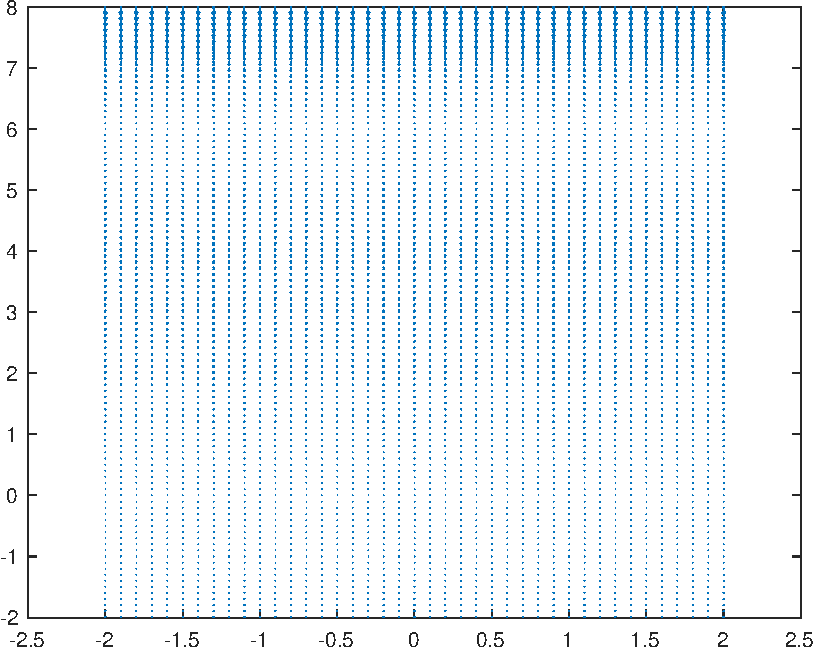
\includegraphics[scale=.8]{IM/B2.pdf}
    \caption{Boceto 1}
    \label{fig=int1}
\end{figure}
        
        Como podemos observar en el boceto de las soluciones $y=6 $ es un punto estable.
\end{enumerate}

\item[b)] $y'=4y^4+4y^3-3y^2$
\begin{enumerate}
    \item Primero factorizamos para encontrar las raíces.
    \begin{align*}
        4y^4+4y^3-3y^2 &= 0 \\
        y^2(4y^2+4y-3) &= 0 \\
        y^2(2y+3)(2y-1) &= 0
    \end{align*}
    Entonces las raíces son:\hspace{.5cm} $y=0$\hspace{.5cm}$y=-\frac{3}{2}$\hspace{.5cm} $y=\frac{1}{2}$\\
        Las cuales son las soluciones de equilibrio de nuestra función.
    \item  Evaluamos en los alrededores de nuestras soluciones de equilibrio para observar como se comporta la derivada en esos puntos, y ver si son positivas o negativas.
    \begin{align*}
        f(1) &= 4(1)^4+4(1)^3-3(1)^2  = 5 > 0\\
        f(\frac{1}{4}) &= -\frac{7}{64} < 0\\
        f(-\frac{1}{2}) &= -1 < 0 \\
        f(-1) &= -3 < 0\\
        f(-2) &= 20 > 0
    \end{align*}
        Y así podemos realizar nuestro boceto donde vemos que tipo de punto son las soluciones de equilibrio.
        \item Boceto y tipos de soluciones de equilibrio
\begin{figure}[H]
    \centering
    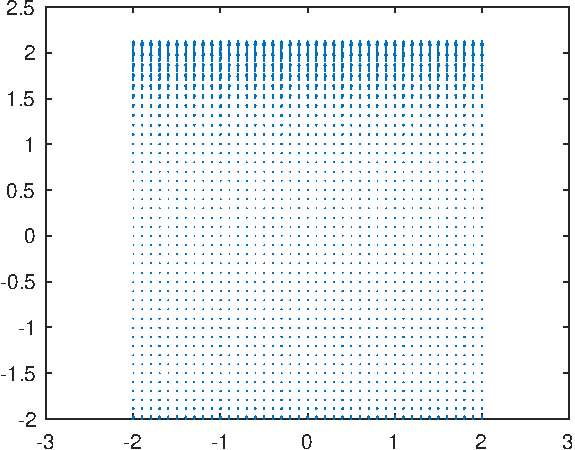
\includegraphics[scale=1.2]{IM/b1.pdf}
    \caption{Boceto 2}
    \label{fig=int1}
\end{figure}
        Como podemos observar en el boceto de las soluciones $y=\frac{1}{2}$ es un punto inestable y $y=-\frac{3}{2}$ es un punto estable.
    
\end{enumerate}

\end{itemize}



\end{document}